\subsection{Hardware and Software Configuration}

The details of the computer were the test was performed,
as the following.

\begin{footnotesize}
\begin{itemize}
	\item CPU: 16 x Intel(R) Xeon(R) CPU E5520  @ 2.27GHz
	\item RAM: 12 GB
	\item Graphic Card: 2 x nVidia Tesla C1060.
	\begin{itemize}
		\item Number of GPUs: 1
		\item Number of GPU cores: 240
		\item Cores frequency: 1.3 GHz
		\item Memory: 4GB
	\end{itemize}
	\item OS: Scientific Linux SL release 5.6 (Boron)
	\item Kernel: 2.6.18-238.12.1.el5 x86\_64 GNU/Linux
\end{itemize}
\end{footnotesize}

\subsection{Execution Set-up}

To the OpenMP and Pthreads implementation
we consider one node with the previous technical details,
and the benchmark was performed using the following combinations:

\begin{center}
\begin{tiny}
\begin{tabular}{|l|r|r|r|r|r|r|r|r|r|}
	\hline
	Number of cores: & 1 & 2 & 4 & 6 & 8 & 10 & 12 & 14 & 16 \\
	\hline
	Number of bodies: & 16 & 32 & 64 & 128 & 256 & 512 & 1024 & 2048 & 4096 \\
	\hline
\end{tabular}
\end{tiny}
\end{center}

For each number of cores, we perform test with all the number of bodies combinations.
Each test, was execute 20 times, to ensure an approximated real value.

In the other hand,
the test on the GPU was performing modifying the number of block per grid (BpG)
and the number of threads per block (TpB), with the constraint
that the warp launch set of 32 threads, so to do not waste threads,
we use threads between 32 and 512, so for each amount of bodies,
we divide it, in multiples of 32 (i.e., for 1024 bodies we use,
(2 BpG, 512 TpB), (4 BpG, 256 TpB), (8 BpG, 128 TpB), (16 BpG, 64 TpB) and
(32 BpG, 32 TpB)) 

\subsection{Assessment on Parallel Performance}

We consider the speed-up to evaluate the performance
in each implementation according to the following formula:

\begin{equation}
Speed\  up\ =\ \frac{Serial\ Time}{Parallel\ Time} \\
\end{equation}

\subsubsection{OpenMP assessment}

In the figure~\ref{fig:openmp} we can see the most representative speed-up of some
amount of bodies.

\begin{figure}[h!t]
    \centering
    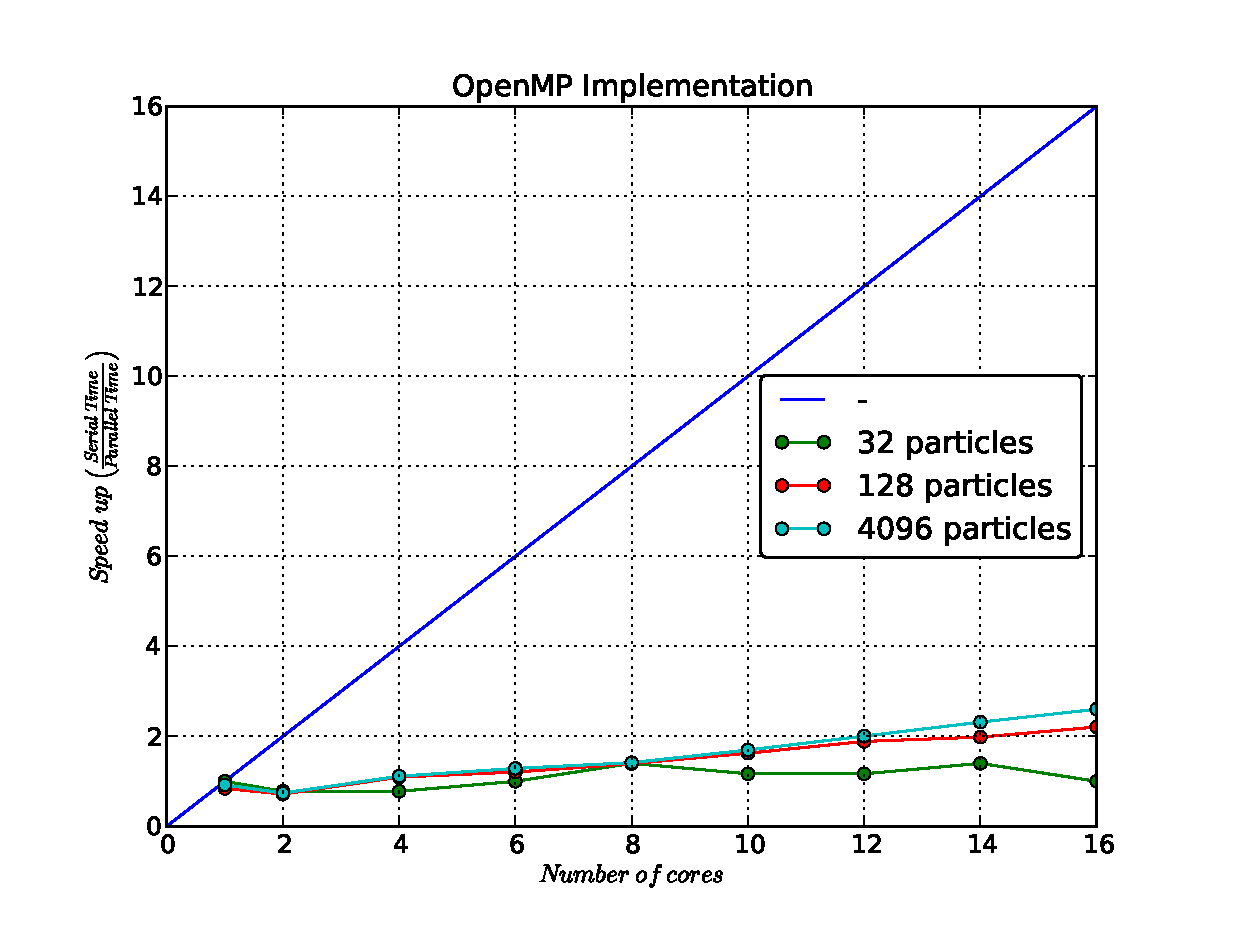
\includegraphics[width=0.5\textwidth]{images/openmp.eps}
    \caption{OpenMP implementation. Speed-up of 32, 128 and 4096 bodies.}
    \label{fig:openmp}
\end{figure}

The difference between the amount of bodies is very big,
and as the figure~\ref{fig:openmp} shows the behaviour in speed-up terms,
is very similar, which represents that the OpenMP implementation works
in the same way, almost independent of the amount of bodies, which is not
a good scenario in this simulation, because it is expected an evolution
considering different bodies amount.

We can not forget that the additional programming with OpenMP
is almost nothing, only one pragma line, and it is possible to obtain
a x3 speed-up.

\subsubsection{Pthreads assessment}

In the figure~\ref{fig:pthread} we can see the most representative speed-up of some
amount of bodies.

\begin{figure}[h!t]
    \centering
    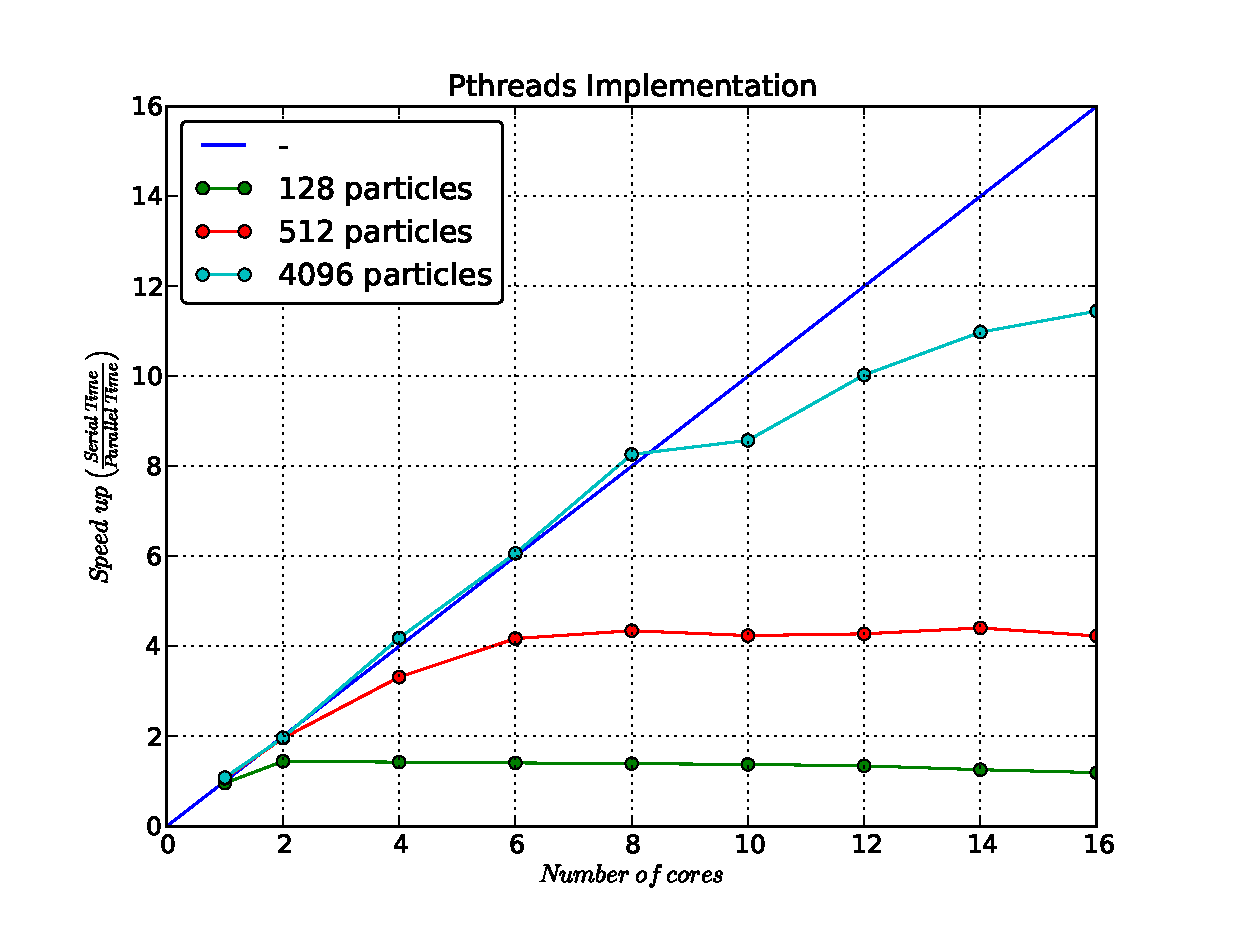
\includegraphics[width=0.5\textwidth]{images/pthreads.eps}
    \caption{Pthreads implementation. Speed-up of 128, 512 and 4096 bodies.}
    \label{fig:pthread}
\end{figure}

In this case, we can note that the normal evolution of the speed-up
considering an increase in the amount of bodies, because with more bodies
we can give more work to each thread, without wasting so much resources.
It is important to remember that in this implementation, there is a little trick
gathering $\frac{n}{c}$ bodies per thread (n: total bodies, c: total cores).

Another important issue, is that the synchronization is performed by the program
itself, in difference with the pre-compilation process used by OpenMP.

Note that the behavior with a little amount of bodies is very similar,
and in both represented cases we can see an asymptotic behavior,
with more than 6 cores.

\subsubsection{CUDA assessment}

In the figure~\ref{fig:cuda} we can see the acceleration factor of all
the performed test, using different numbers of bodies.

\begin{figure}[h!t]
    \centering
    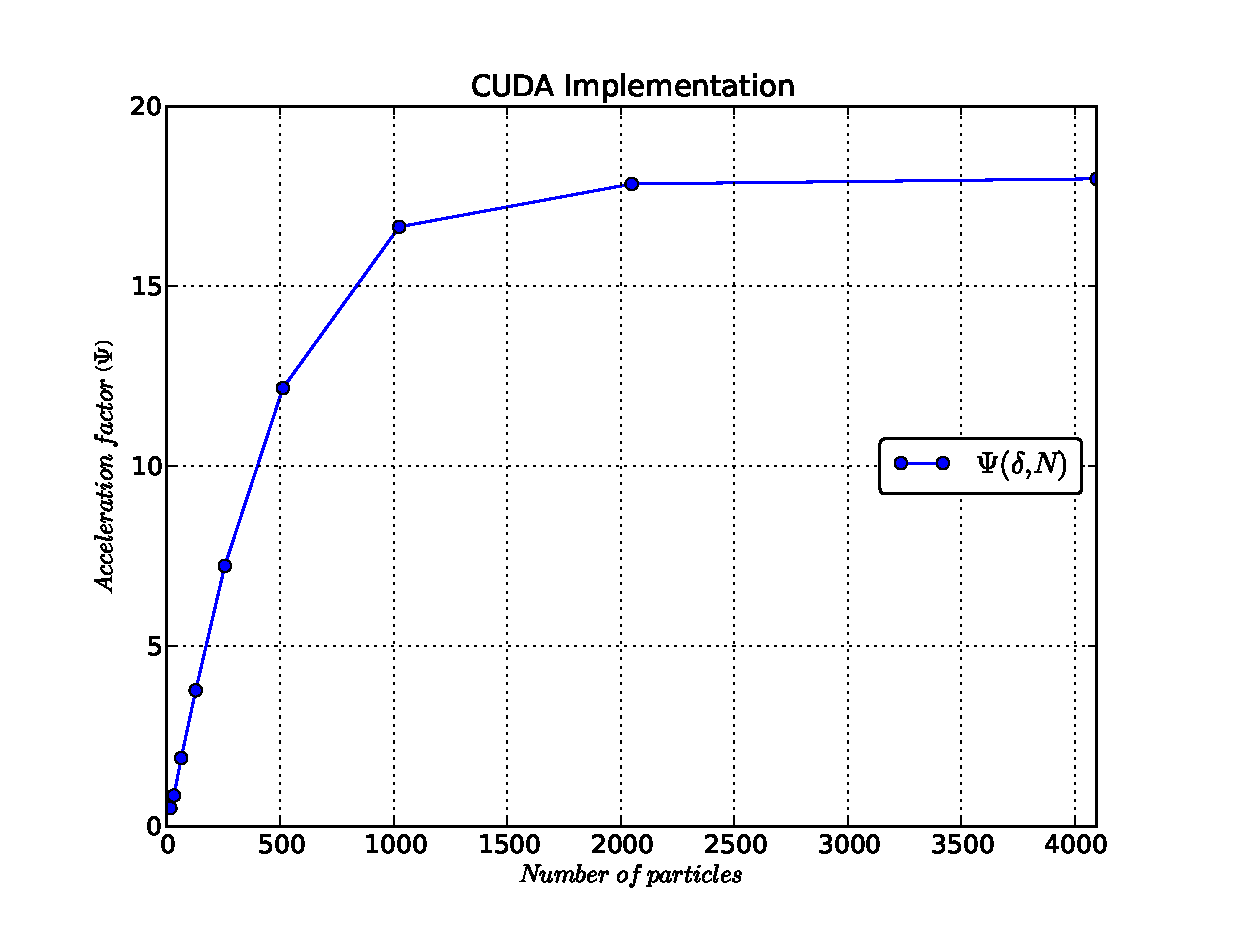
\includegraphics[width=0.5\textwidth]{images/cuda.eps}
    %\caption{CUDA implementation.\\ Acceleration factor of 16, 32, 64, 128, 256, 512, 1024, 2048 and 4096 bodies.}
    \label{fig:cuda}
\end{figure}

This case can be seen as a different implementation,
considering the huge difference between the CPU cores and the GPU cores,
following the previous idea, we present an Acceleration Factor to represent the speed-up on GPU,

\begin{eqnarray}
    \Psi(\delta,N) = \dfrac{t_{s}}{t_{p_{(\delta)}}} 
\end{eqnarray}

the main idea is the same, serial time versus parallel time,
but in each GPU iteration we use a configuration ($\delta$) between the
\emph{blocks per grid (BpG)} and the \emph{threads per block (TpB)},
aside of the fixed number of GPU cores.

In the figure~\ref{fig:cuda} we can appreciate
the behavior of the CUDA implementation increasing the amount of bodies,
obtaining a really good acceleration factor,
but after the 2000 bodies, it is possible to note
a asymptotic behavior, which shows an issue in the implementation,
breaking the initial good scalability.

\begin{figure}[h!t]
    \centering
    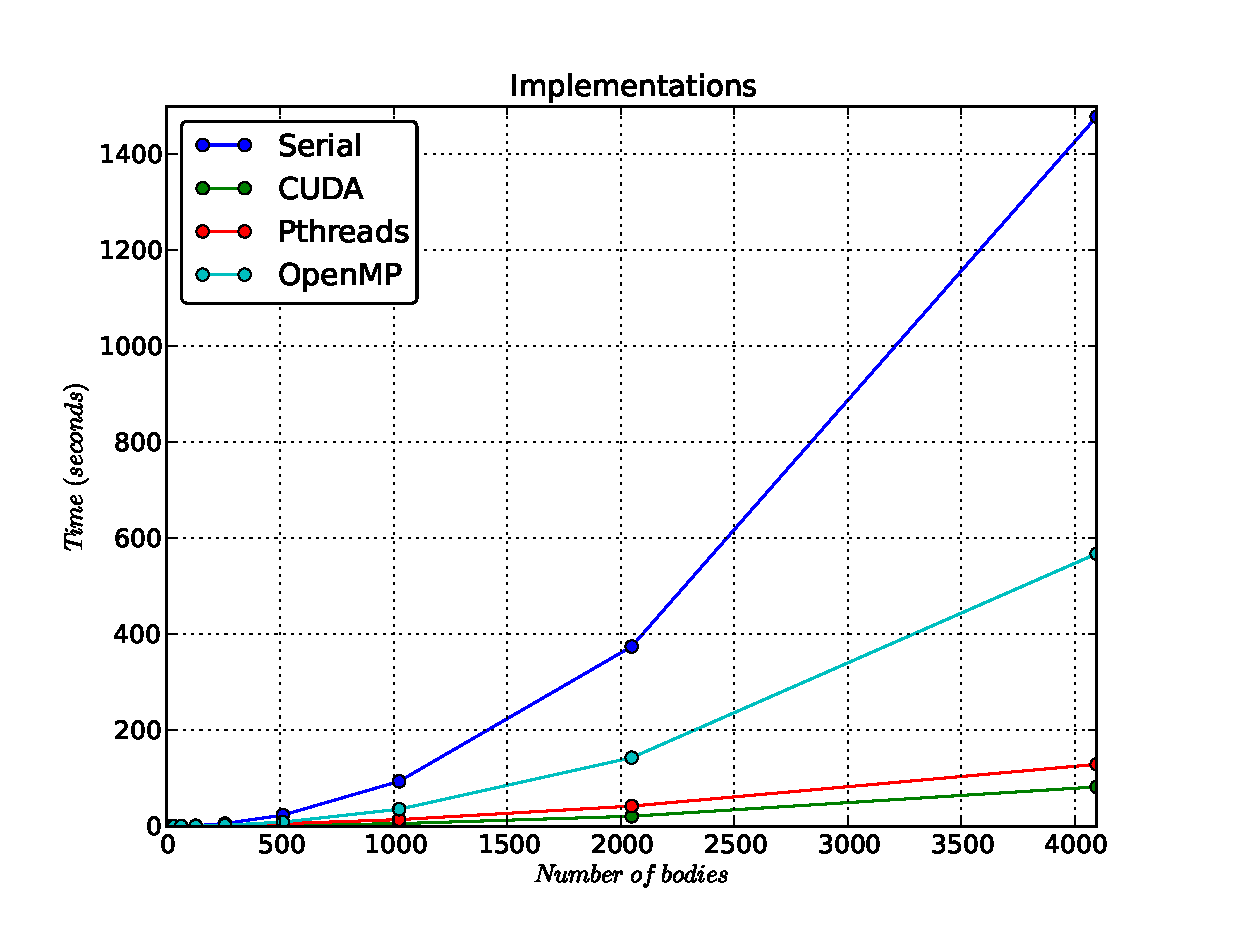
\includegraphics[width=0.5\textwidth]{images/all.eps}
    \caption{Best execution time of each implementation.}
    \label{fig:all}
\end{figure}

Finally, as the figure~\ref{fig:all} and the table~\ref{tab:all} shows,
the final review of each technique is very clear.

Understanding the differences between the CPU and GPU
programming paradigms, is good to consider both alternatives
at the time to solve problems with a large computational work.

\begin{table}[h!t]
    \centering
    \begin{tabular}{|c|c|}
        \hline
        \textbf{Implementation} & \textbf{Speed-up} \\\hline
        Serial  & 1x  \\\hline
        OpenMP  & 3x  \\\hline
        Pthreads & 11x \\\hline
        CUDA    & 18x \\\hline
    \end{tabular}
    \label{tab:all}
    \caption{Final best results of the performed tests}
\end{table}

Please note, that not always the CUDA implementation
will be the best, this happens only because this algorithm,
is \emph{fine-grained}, and the CPU are a best choice for
\emph{coarse-grained} algorithms, which is affirmed
by the Pthreads results, because the transformation
in the code, gathering bodies to give more work to the CPU,
changing from fine to coarse grain.
